\chapter{Final Solution}
\label{chp:5:FinaSolu}
In this chapter, a final design of a mass communication system, named Myriad, will be introduced. Firstly, the improvements on the requirements will be compared to the ones defined for the prototype from previous chapter. Later, the actual product's features, and its architecture will be discussed.

\section{Improved Requirements}
\label{sec:5.1:ImprRequ}

Having seen the prototype in action made us to review the requirements, and bring the ones. Some of those requirements are shaped according to the feedbacks that we got at the Stanford \ac{HCI} group, as well as the organizations who do mass email communication on weekly basis to reach their community. Following sections will discussed those new features on the final product. 

\subsection{Assistant Support}
\label{subsec:5.1.1:AssiSupp}
As it it discussed in section \ref{subsec:4.1.1:Cust}, the standard that we want to achieve within a mass email communication is the most adequately personalized emails according to recipients with minimum effort on a researcher's side. The initial idea and the prototype brought several features as discussed in chapter \ref{chp:4:InitIdeaProt} for this purpose. However, if you consider the gold standard in the figure \ref{fig:ChartEffortCustom} we would like to achieve, the prototype still leaves effort on a researcher to accomplished a successful mass email campaign.
\vspace{1cm}

In order to minimize the efforts on the researcher's side, the additional assistants' involvement was considered. Therefore, a primary researcher will be able to share the tasks with permitted assistants. These tasks may be extracting information from the incoming answers or even writing replies to those answers. Hence, the primary researcher will only need to interact with the flow of a mass email campaign when there is situation where it requires primary researcher attention. However, the system still needs to provide the necessary features that we will see in the next sections to support the work flow in a mass email campaign, hence assistants will only need to interact with this work flow to let the continuation of the email campaign by providing answers with the email templates, and extract information as \ac{KVP}s.

\subsection{Dynamic Variables and \ac{KVP}s}
\label{subsec:5.1.2:DynmVariKVPs}
We introduced dynamic variables at the initial prototype, however it was only limited at the salutation of the email. Since it allows the personalization of emails easier, and email marketing applications also supports this feature in the same purpose in section \ref{subsec:3.3.3:EmaiMarktAppl}, the final product will also include this feature. As a result, application users can create \ac{KVP}s and use those keys in the content of the email message to be replaced dynamically by its value according to the recipients. Therefore, the extracted information from the emails will not just help us to gather information in an organized, but also use them to personalize the emails
\vspace{1cm}

As a result, instead of keeping the \ac{KVP}s in the system according to the responds, system should keep them according to the recipients itself. This is where the \ac{KVP}-idea differs from the prototype as well. So, we have now profiles of contacts for a campaign having all \ac{KVP}s of a recipients visible during the whole state of the conversation, not just at one message of the recipient. However, system should offer an option to hide individual \ac{KVP}s to avoid cluttering on the view, and keep the \ac{KVP} list with the ones that are actively used.

\vspace{1cm}
Importing the \ac{KVP}s should be done in several ways. One option is that system should be able to synchronize with an online spreadsheet, e.g. Google Spreadsheet, to get the \ac{KVP}s at the beginning of a campaign. This is a convenient way for the researchers since they are already familiar with spreadsheet environment. Other options should be a campaign-wide view and a contact specific view in the system. Also, system should allow to edit both keys and values in a campaign.

\subsection{Importing and Exporting Contacts and Their Information}
\label{subsec:5.1.3:ImpoExpoContInfo}
In the prototype, application user had to enter the basic information of the recipients such as first name, last name, and email address into the system manually. However, we realized while they were doing this, they use a spreadsheet and copy the contact information from there. This was also the case for their regular email client that they used for email campaigns. The applications that was investigated in section \ref{sec:3.3:Resul} had an option to import from spreadsheet to ease the process. Therefore, the system should offer an option to import contacts from the spreadsheet environment.
\vspace{1cm}

However, importing should not be limited only the basic information of the recipients. Since we already mentioned about importing \ac{KVP}s from spreadsheet in the previous section, system should detect and import the contact information and \ac{KVP}s related to that contact if it is available from a provided spreadsheet. 
\vspace{1cm}

System should provide a bi-directional synchronization, not just importing data from the spreadsheet. Therefore, system should provide an option to export contact information and their created \ac{KVP}s from the system to the spreadsheet. This will also gives a reporting functionality to the application users, where they can see all the contacts, and their extracted information from a campaign in one view.

\subsection{Interoperability with Other Email Clients}
\label{subsec:5.1.4:InteEmaiClie}
Even though we provide a new system for the users to conduct their mass email communication, there might be some cases where a mass email communication initiated in the user's regular email client, and the system is not aware of that campaign since it was not created with it. Application should provide an option to import those emails messages created with another email client in to the system by recognizing those annotated messages by the user.
\vspace{1cm}

Enabling the system to import email conversations from other email clients reduce the dependency on the application, and while a researcher continue to use their own email client, assigned assistants can take care of those imported emails by the researcher. We saw such a import feature in \ac{CRM} applications in section \ref{subsec:3.3.1:CRMAppl} as well, where a user is able to forward an email into the \ac{CRM} application, and system takes care of assigning the imported email to the corresponding recipient entry in the system.

\subsection{Automated Decision-Making and Notifications}
\label{subsec:5.1.5:AutoDeciMakiNoti}
Even though the involvement of assistants make the initial researcher's life easier, the system still needs to provide an automated approach to answer the emails whose status is clear in the flow of a mass email communication. Therefore, a rule based decision-making mechanism should be used, where users sets the values of the keys of \ac{KVP}s, and it triggers the action of sending an email to a respondent.
\vspace{1cm}

Since the application's only purpose is the managing mass email communication and each campaign results great amount of messages in the inbox, the system should provide notifications regarding what should be done next for each recipients. Labels added to the email conversation should state whose turn is next in the communication. For instance, by proving a label saying "You need to reply" to the application user, the state of the communication waits an action from a researcher or an assistant. In the same way the unread conversations and the conversation waiting an answer from the respondents should be also annotated in the similar fashion. System should also provide email notification to the assistants' email addresses to notify them there is an action waiting to be taken care of.

\section{Final System}
\label{sec:5.2:FinaSyst}
In this section, we will see that how the revised and improved requirements from section \ref{sec:5.1:ImprRequ} reflected to the final product, named "Myriad".

\subsection{Log-In and Campaigns Overview}
\label{subsec:5.2.1:CampOver}

As it was the same case for the prototype in section \ref{subsec:4.2.2:ProtSyst}, Myriad also requires a Gmail account to work with. the reason behind is not just the popularity of the Gmail, but also Stanford University uses Google Apps by default. Therefore, each member of the university has a Google account to use with Myriad. This also provides flexibility to use Myriad, because there  is no registration form or sign in screen.
\vspace{1cm}

After user sign in to the system, the first screen that they will see is the campaigns overview screen, in where all the created campaigns including the ones that are shared with the user (as a assistant) are shown as in the figure \ref{fig:CampaignsOverviewScreen}. It has a simple and a clean \ac{UI}, deferring from regular email clients to emphasize its focus on mass email communication.

\begin{figure}[htbp]
	\centering
	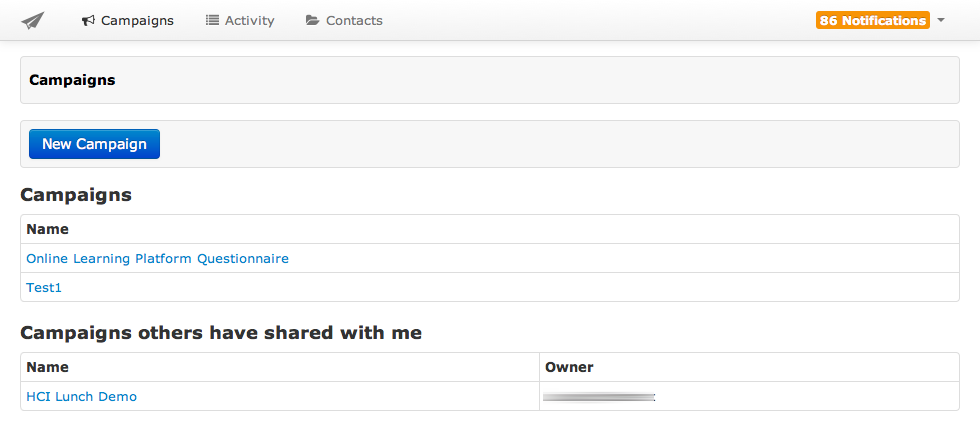
\includegraphics[width=1.00\textwidth]{imgs/CampaignsOverviewScreen.png}
	\caption[Myriad's Campaigns Overview Screen]{Myriad's Campaigns Overview Screen}
	\label{fig:CampaignsOverviewScreen}
\end{figure}

\subsection{Synchronization with Other Sytems}
\label{subsec:5.2.2:SyncOtheSyst}

Myriad is able to get the contacts' information and their \ac{KVP}s from Google Spreadsheet. This is a convenient way to import contacts into the system since many people already keeps their information in a spreadsheet environment as we discussed in section \ref{subsec:5.1.3:ImpoExpoContInfo}. Therefore, Myriad offers a bi-directional syncing from and to the spreadsheet defined at the creation of a campaign. Besides, Myriad also offers an option to enter recipients first name, last name, and email address into the system directly.
\vspace{1cm}

The corresponding columns in the spreadsheet start with "first name", "last name", and "email address" as in the figure \ref{fig:GoogleSpreadsheet}. The rest of the columns will be acted as a \ac{KVP}, and imported into the system as well.

\begin{figure}[htbp]
	\centering
	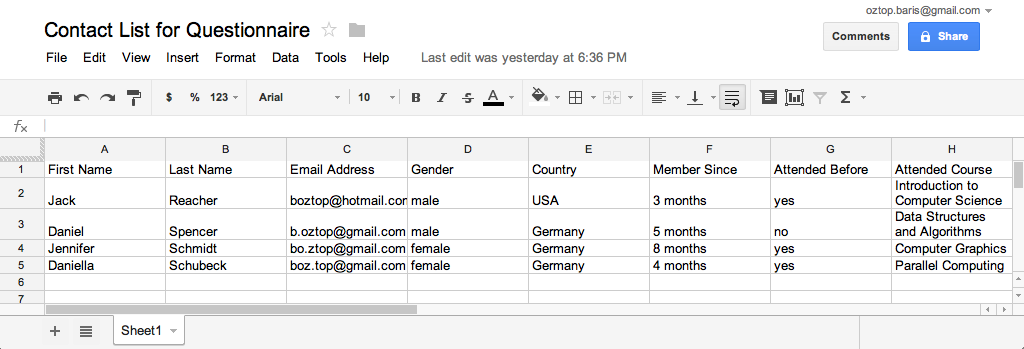
\includegraphics[width=1.00\textwidth]{imgs/GoogleSpreadsheet.png}
	\caption[A Google Spreadsheet to Import into Myriad]{A Google Spreadsheet to Import into Myriad}
	\label{fig:GoogleSpreadsheet}
\end{figure}

As it was discussed in section \ref{subsec:5.1.4:InteEmaiClie}, importing existing email conversations as campaigns into the system is an important feature, since researchers may initiate conversations in their regular email client, and later on to make them more manageable, they can import them into Myriad. Myriad leverages Gmail's labeling feature which is equivalent to the \ac{IMAP} protocol's folders for this purpose \citep{GoogleInc.2013}. Myriad creates a Gmail label in the user's account, and the only thing that user needs to do is the enable label syncing feature at the create campaign screen. Next, there will appear a label with the campaign name, and group under the root label of "myriad" in Gmail's inbox as in the figure \ref{fig:GmailLabels}. Hence, researcher will able to imports email messages, which were not considered to belong to a campaign for some reason, into Myriad.

\begin{figure}[htbp]
	\centering
	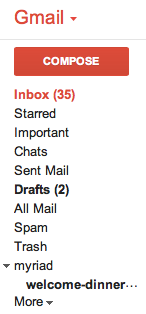
\includegraphics[scale=0.60]{imgs/GmailLabels.png}
	\caption[Gmail's Labels and the Myriad's Campaigns Under the Myriad Label]{Gmail's Labels and the Myriad's Campaigns Under the Myriad Label}
	\label{fig:GmailLabels}
\end{figure}

\subsection{Creating an Email Campaign}
\label{subsec:5.2.3:CreaEmaiCamp}

The campaign creation screen (see figure \ref{fig:CreateCampaign}) has input fields for a campaign name and Google Spreadsheet's URL to synchronize with. Other two checkboxes for the spreadsheet are to manage the frequency of synchronization and disabling the warning in case of erroneous data in the spreadsheet such as an empty email address field for a contact. The option for importing emails from Gmail's inbox is also in this screen under label synching.

\begin{figure}[htbp]
	\centering
	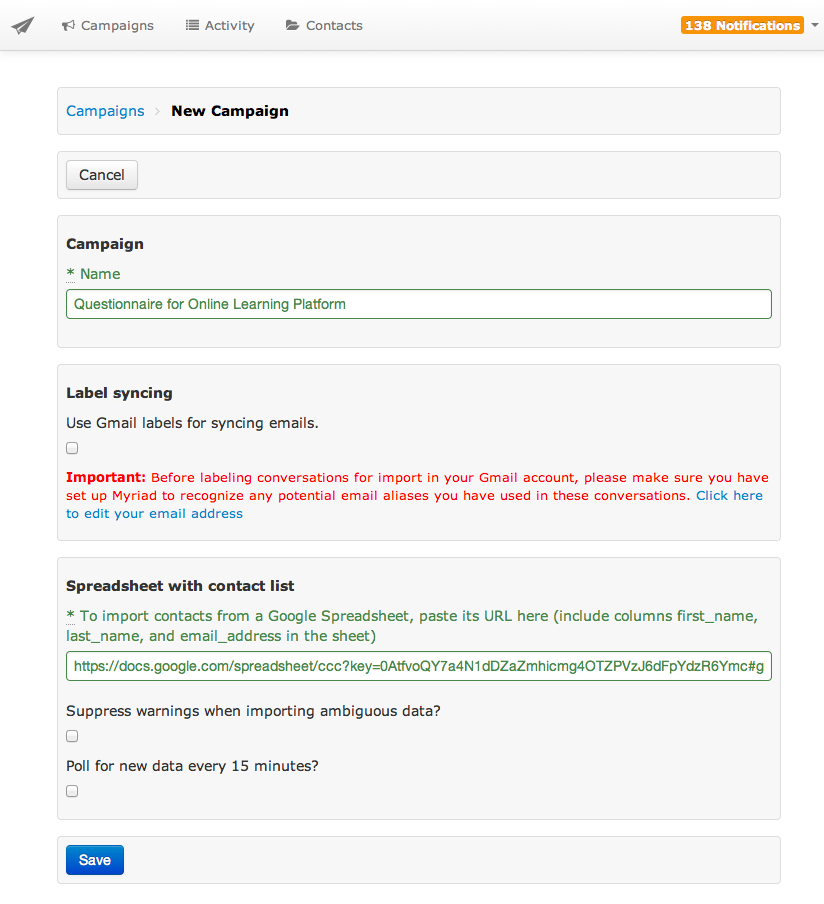
\includegraphics[width=1.00\textwidth]{imgs/CreateCampaign.png}
	\caption[Creating a Campaing in Myriad]{Creating a Campaing in Myriad}
	\label{fig:CreateCampaign}
\end{figure}

After the campaign is created, all the contacts and their \ac{KVP}s will imported if the user provided a Google Spreadsheet as in the figure \ref{fig:ContactListInCampaign}.

\begin{figure}[htbp]
	\centering
	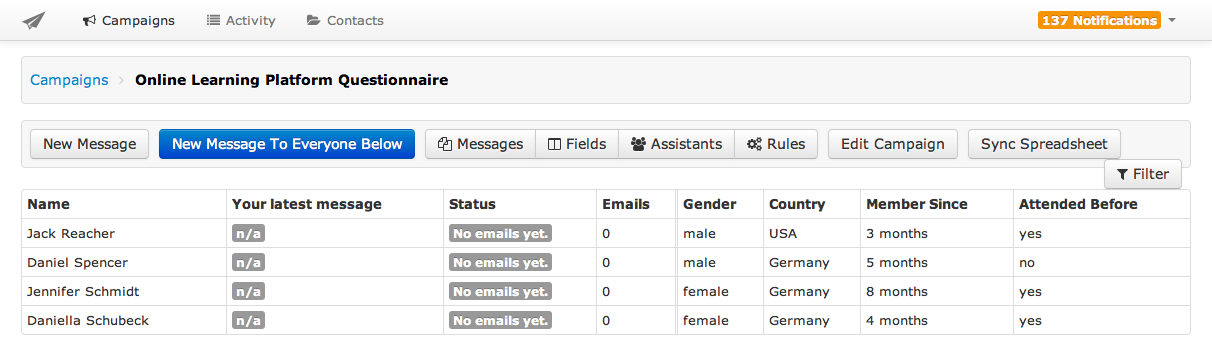
\includegraphics[width=1.00\textwidth]{imgs/ContactListInCampaign.png}
	\caption[Contacts and Their \ac{KVP}s After Synchronization in Myriad]{Contacts and Their \ac{KVP}s After Synchronization in Myriad}
	\label{fig:ContactListInCampaign}
\end{figure}

\subsection{Composing an Email Message}
\label{subsec:5.2.4:CompEmaiMess}

Users can send emails to all the contacts that they entered or imported into the system, or select a subset of it by using the filtering functionality as in figure \ref{fig:ContactFilters}. Provided filtering option are according to values of \ac{KVP}s, conversation status such as unread, replied, or unreplied, or the last message's template name.

\begin{figure}[htbp]
	\centering
	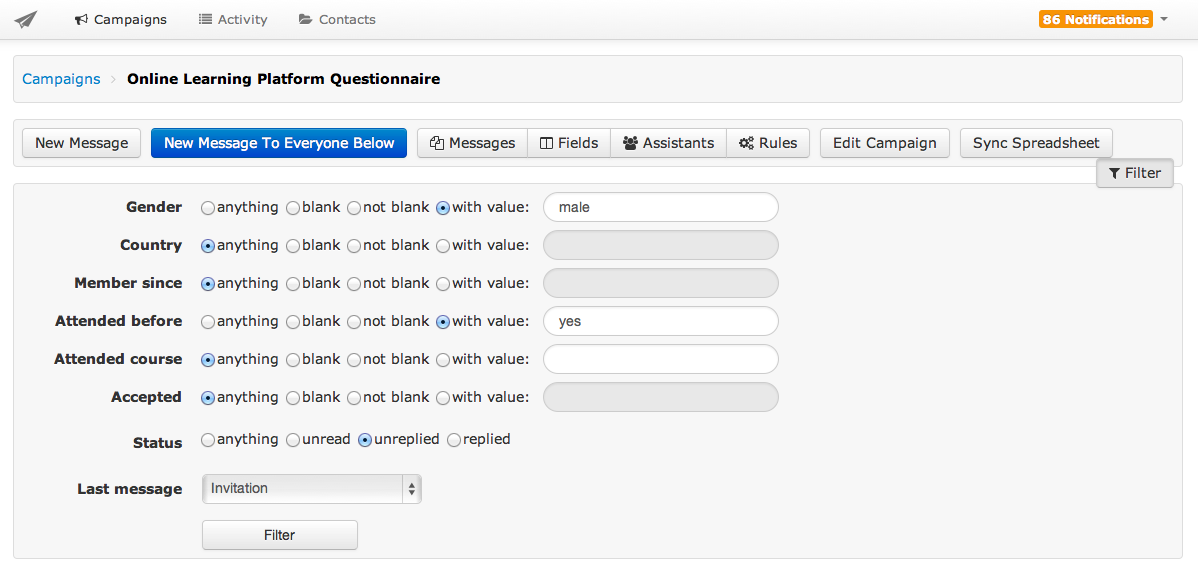
\includegraphics[width=1.00\textwidth]{imgs/ContactFilters.png}
	\caption[Filtering the Contact List in Myriad]{Filtering the Contact List in Myriad}
	\label{fig:ContactFilters}
\end{figure}

Filtered recipients are ready to be composed of email at the compose screen after pressing the corresponding button. The compose email pane (see figure \ref{fig:ComposeEmail}) contains a section that lists the previously sent emails to reuse. This is the same templating idea that was introduced at the prototype in chapter \ref{chp:4:InitIdeaProt} section \ref{subsec:4.2.2:ProtSyst}. It also shows the visualization of the state of the communication by using a tree structure, as well as the number of messages sent by using the corresponding template. A more long term campaign's visualization tree can be found in appendix \ref{app:VisuCommStat}.

\begin{figure}[htbp]
	\centering
	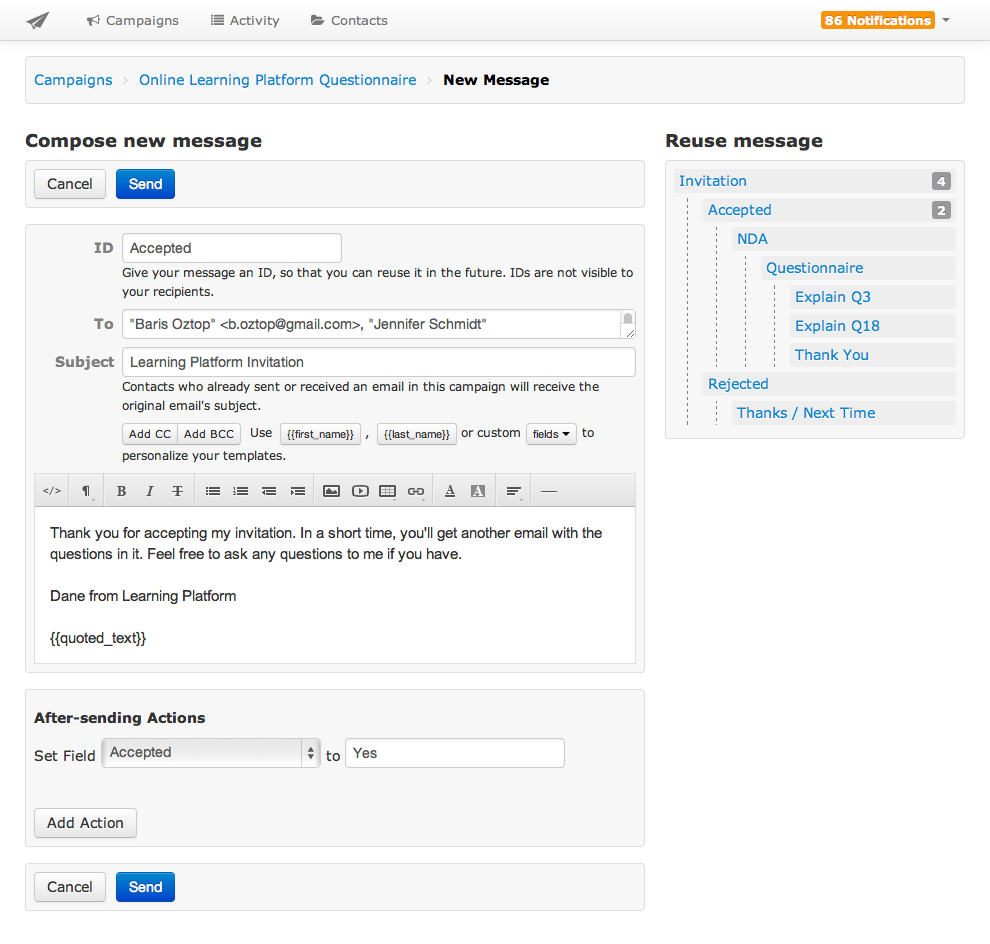
\includegraphics[width=1.00\textwidth]{imgs/ComposeEmail.png}
	\caption[Compose an Email in Myriad by Reusing Earlier Messages]{Compose an Email in Myriad by Reusing Earlier Messages}
	\label{fig:ComposeEmail}
\end{figure}

The compose pane allows users to dynamic variables into the content of messages to personalize them according to recipients. Those variables are not just limited to the first name and last name, but also can be any keys from the assigned \ac{KVP}s in the campaign.
\vspace{1cm}

\ac{KVP}s are accessible among different campaigns, therefore extracted information from an earlier campaign can be used in a new campaign as well. Having broader knowledge about a recipient may help  researchers personalize the content of the emails more easily and properly. For example, if we had extracted information regarding which sports that the recipients do in an earlier campaign. We can use the same information to make a more frankly and friendly start in the new campaign by mentioning about the latest events of those sports areas in the country. Such a technique also supports the social exchange and the diffusion of responsibility theories as discussed in section \ref{sec:2.3:PersEmai}. There is also an option to hide the \ac{KVP}s in a campaign if they are not related at all or became obsolete during the flow of the campaign to avoid cluttering of \ac{KVP}s in the application's view.
\vspace{1cm}

In the figure \ref{fig:ComposeEmail}, under the section of after-sending actions, users are able to set the values of the keys right after an email is sent. Therefore, a user does not need to browse another screen to change or set \ac{KVP}s whose values depends on the email user has just sent.
\vspace{1cm}

At the beginning of this section it is mentioned that a user can filter the recipients list, and send an email to the subset of it according to filtered condition. Myriad saves those filtered condition under the "Rules" menu as in the figure \ref{fig:AutomatedRules} after the user sent the email. Hence, the next time if there are new emails satisfying the same conditions as before, user will notice them under the rules menu, and the earlier sent email message can be sent to those new matching recipients automatically if user chose to enable it automated option or a user can simple press the send button manually in the same screen. For example, it the figure \ref{fig:AutomatedRules}, there are 3 recipients whose "attending" key was set to "yes", and the system already recognized that we already sent an email to those whose attending, and there are new matches for the same condition. In this case, the user can simply press the send button after, or automated the process by enabling the provided option.

\begin{figure}[htbp]
	\centering
	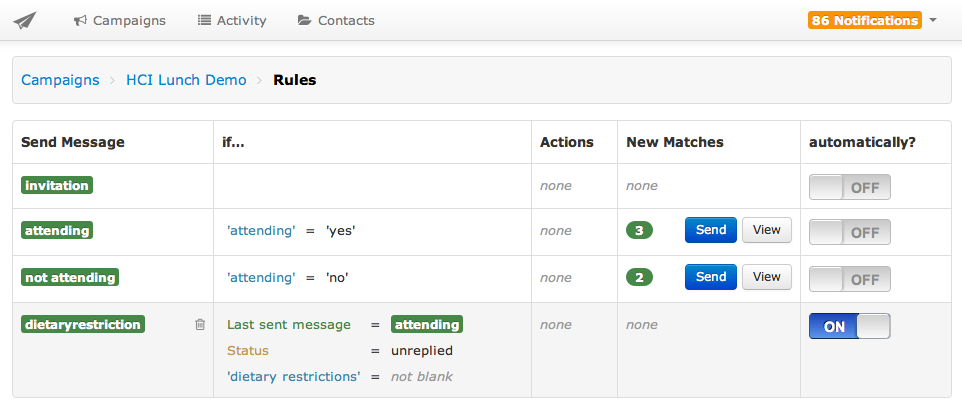
\includegraphics[width=1.00\textwidth]{imgs/AutomatedRules.png}
	\caption[Rules to Automate the Sending Process of the Emails in Myriad]{Rules to Automate the Sending Process of the Emails in Myriad}
	\label{fig:AutomatedRules}
\end{figure}

\subsection{Extracting Information from Email Messages}
\label{subsec:5.2.5:ExtrInfoEmaiMess}

Myriad's reading pane (see figure \ref{fig:MyriadReadingPane}) offers a threaded view for all the messages of a recipient in a campaign. Each of the researcher's message is also annotated with the name of the message template that was used to make the latest state of the communication can easily recognizable.

\begin{figure}[htbp]
	\centering
	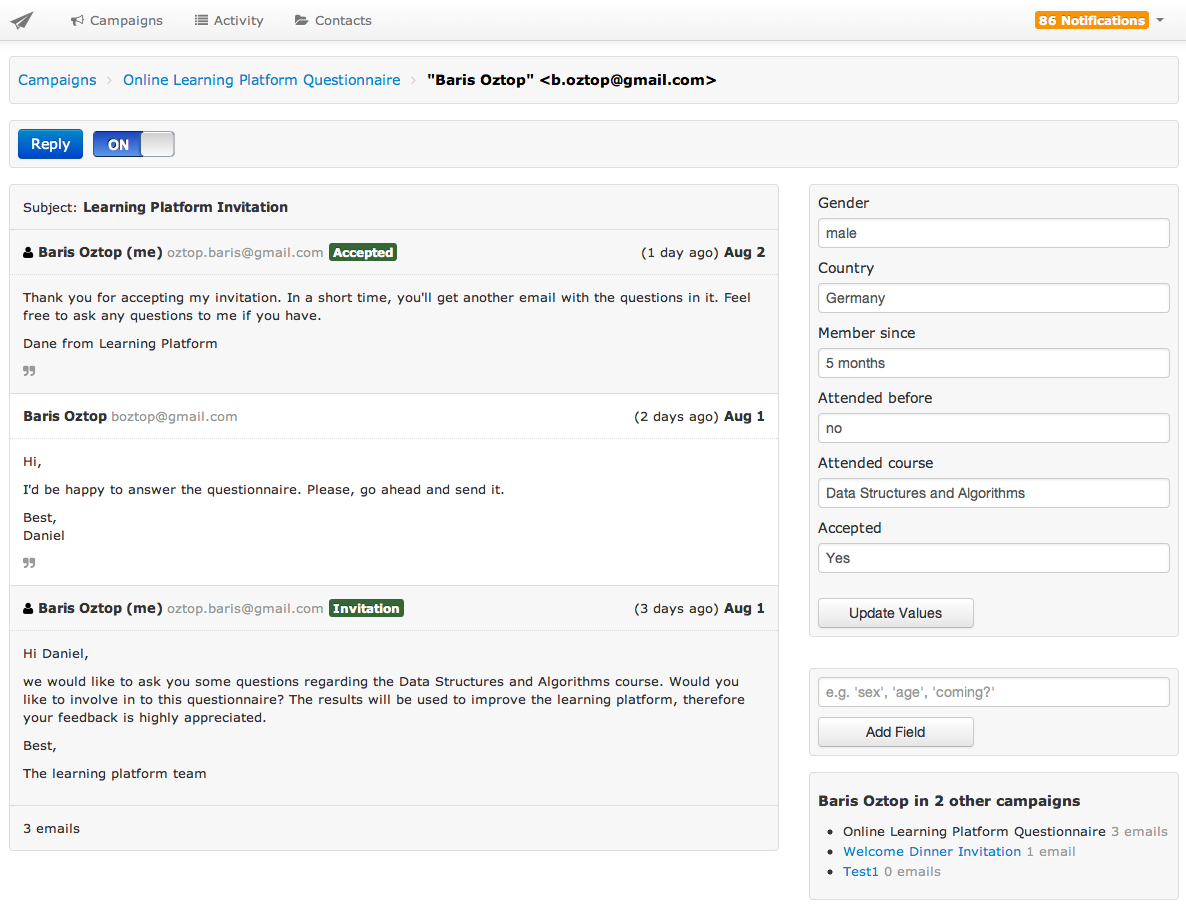
\includegraphics[width=1.00\textwidth]{imgs/MyriadReadingPane.png}
	\caption[Reading Pane and Extracted \ac{KVP}s in Myriad]{Reading Pane and Extracted \ac{KVP}s in Myriad}
	\label{fig:MyriadReadingPane}
\end{figure}

\subsection{Enabling Assistants}
\label{subsec:5.2.6:EnabAssi}

A researcher can add other researchers as assistants into a campaign by adding their Google account email addresses into Myriad as in the figure \ref{fig:AddAssistants}. The task of a researcher can be extracting information from the email, writing answer to the recipients, or even proofreading of a researcher's emails before sending them.

\begin{figure}[htbp]
	\centering
	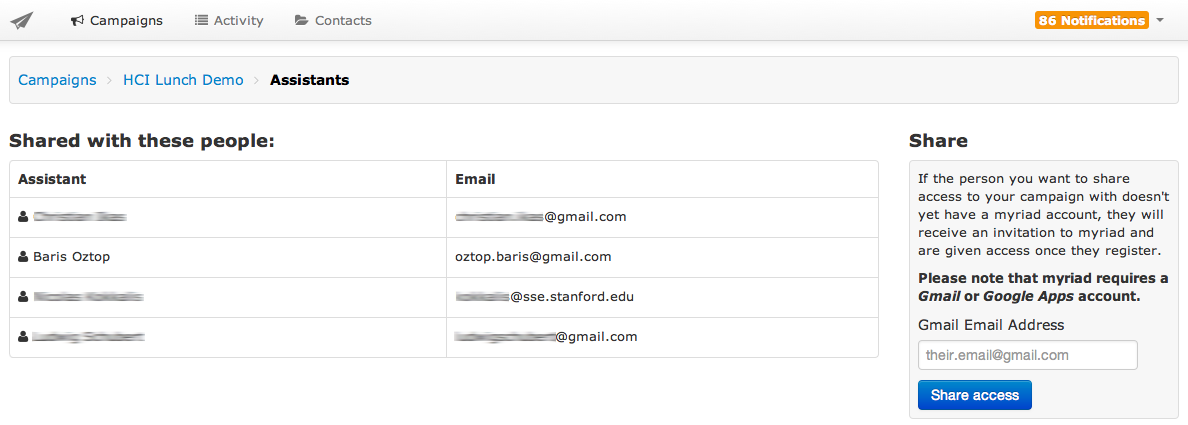
\includegraphics[width=1.00\textwidth]{imgs/AddAssistants.png}
	\caption[Rules to Automate the Sending Process of the Emails in Myriad]{Rules to Automate the Sending Process of the Emails in Myriad}
	\label{fig:AddAssistants}
\end{figure}

After an assistant is assigned to a campaign, he or she will get an notification email including the link to the campaign. Again, there will be a notification email for each email coming from respondents to the assistants' email address to let them know about the action required situation.
\vspace{1cm}

Myriad provides status labels for each received or sent email to give a hint about the next required actions as in the figure \ref{fig:EmailStatuses}. These status labels give a hint about the next action that should be done in the state the conversation such as if the application user needs to read or reply a message, or the action is required from the recipient's side to continue the communication. There are also status labels related with Myriad's internal state regarding to an email message such as if Myriad sent the messages, or there was a failure with sending. The same view also provides a column to show what was the last message that is sent by an application user. Therefore, researchers and assistants will easily realize what should be done next, and see the status of the communication for each recipient. 

\begin{figure}[htbp]
	\centering
	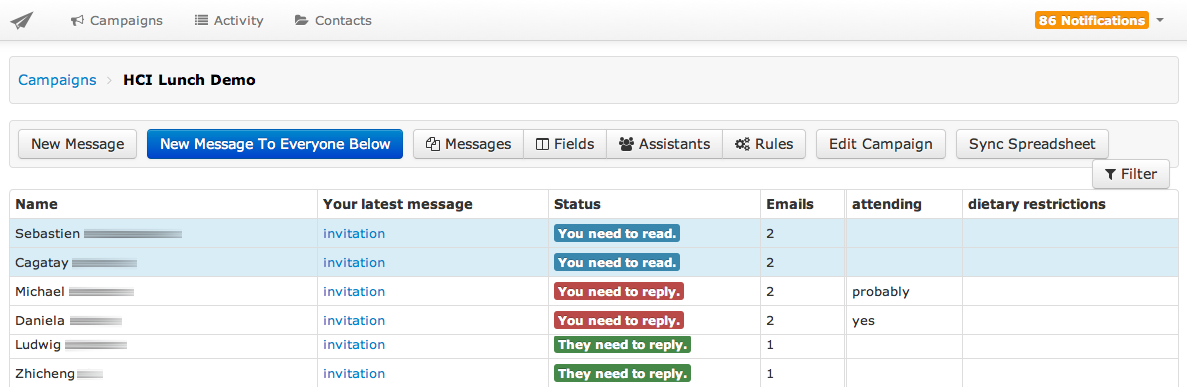
\includegraphics[width=1.00\textwidth]{imgs/EmailStatuses.png}
	\caption[Status Labels for Each Email in Myriad]{Status Labels for Each Email in Myriad}
	\label{fig:EmailStatuses}
\end{figure}

\section{Architecture}
\label{sec:5.3:FinaArch}

\section{Conclusion}
\label{sec:5.4:Conc}

\section{Experiences}
\label{sec:5.5:Expr}

\begin{comment}

--> Gmail labellari ni anlatirken, diger urunlerde import nasil email forwardingle yapiliyordu onu anlat kesin.


However, we still needs to supply a system, where it offers a work flow to make it happen. satisfy these 

distribution of the work

initial idea is reducing effort as we disscussed


Requirements'dan once urunu tanit screenshot'larla cunku cok zaman kaybedecen


write first about the revised requirements,
then describe the product with pictures,
then some technical details

\section{Product}
\label{sec:5.1:FinaProd}

\subsection{Improved Requirements}
\label{subsec:5.1.1:Cust}

\subsection{Final System}
\label{subsec:5.1.2:FinaSyst}

\subsection{Architecture}
\label{subsec:5.1.3:FinaArch}

-------------
chapter 6
-------------
Evaluation
- Experiences
- Statistics
- Conclusion

\end{comment}
